\documentclass[border=3pt]{standalone}
% Preâmbulo compartilhado pelos diagramas TikZ da aula 11 (Localização por Grade e Monte Carlo)
\usepackage[T1]{fontenc}
\usepackage[utf8]{inputenc}
\usepackage{lmodern}
\usepackage{amsmath}
\usepackage{xcolor}
\usepackage{tikz}
\usetikzlibrary{arrows.meta,angles,quotes,decorations.pathmorphing,calc,
                positioning,shapes.geometric,shapes.misc,backgrounds,fit,
                math}

% Paleta (mesma dos SVGs originais)
\definecolor{dblue}{HTML}{2A5B8C}
\definecolor{dorange}{HTML}{B3541E}
\definecolor{dgreen}{HTML}{4A7C59}
\definecolor{dred}{HTML}{9C4B4B}
\definecolor{dcream}{HTML}{F4F1EA}
\definecolor{dshade}{HTML}{DDD7C9}

% Função gaussiana (não normalizada por padrão de escala visual)
\pgfmathdeclarefunction{gauss}{3}{%
  \pgfmathparse{1/(#3*sqrt(2*pi))*exp(-((#1-#2)^2)/(2*#3^2))}%
}

% Estilos comuns (prefixo d... para não colidir com chaves internas do pgf)
\tikzset{
  >={Stealth[length=2mm]},
  dguide/.style={gray!55, dashed, line width=0.4pt},
  daxis/.style={gray!60, line width=0.7pt, ->},
  dbody/.style={fill=black!3, draw=black!80, line width=1pt},
  dacc/.style={draw=dblue, line width=1pt},
  dlbl/.style={black!55, font=\small},
  dsub/.style={black!45, font=\footnotesize},
  dstate/.style={circle, draw=black!80, fill=dcream, line width=1pt,
                 minimum size=17mm, font=\large, inner sep=1pt},
  dobs/.style={circle, draw=black!80, fill=dshade, line width=1pt,
               minimum size=14mm, font=\large, inner sep=1pt},
  dbox/.style={rounded corners=2pt, draw=black!80, fill=dcream, line width=1pt,
               align=center, inner sep=6pt},
  dop/.style={circle, draw=black!80, fill=white, line width=1pt,
              minimum size=6mm, inner sep=0pt, font=\small},
  dtrans/.style={->, dblue, line width=1pt},
  dmeas/.style={->, dorange, line width=1pt},
  dcurve/.style={line width=1pt, dblue},
  dcurveb/.style={line width=1.4pt, dorange},
}

\begin{document}
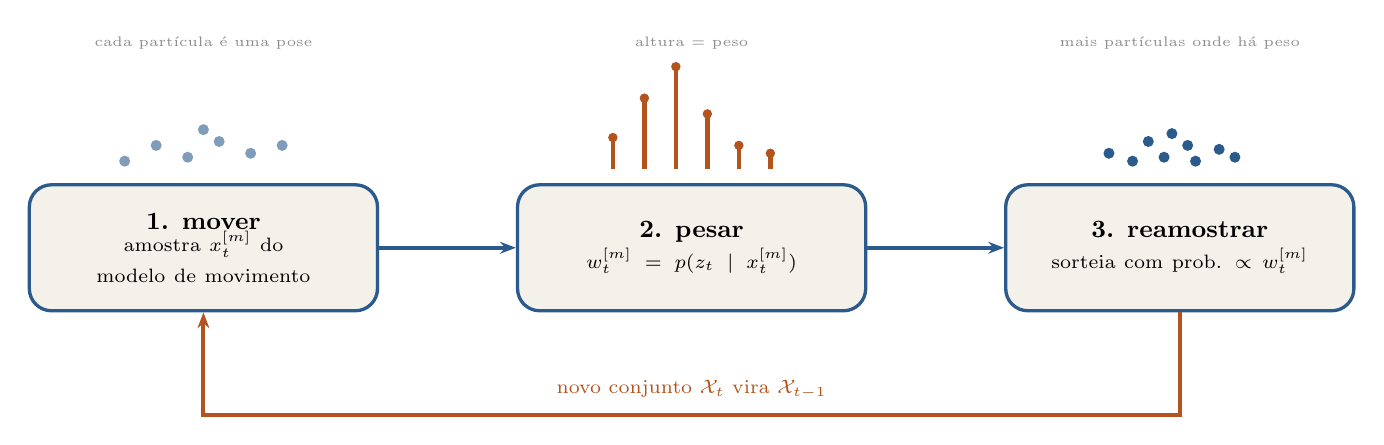
\begin{tikzpicture}[x=1cm,y=1cm,
   st/.style={dbox, rounded corners=8pt, text width=4.0cm, minimum height=1.6cm, font=\small, draw=dblue, line width=1.2pt}]
  \node[st] (a) at (0,0) {\textbf{1. mover}\\ \scriptsize amostra $x_t^{[m]}$ do\\ \scriptsize modelo de movimento};
  \node[st] (b) at (6.2,0) {\textbf{2. pesar}\\ \scriptsize $w_t^{[m]} = p(z_t \mid x_t^{[m]})$};
  \node[st] (c) at (12.4,0) {\textbf{3. reamostrar}\\ \scriptsize sorteia com prob. $\propto w_t^{[m]}$};
  \draw[dtrans, line width=1.4pt] (a) -- (b); \draw[dtrans, line width=1.4pt] (b) -- (c);
  \draw[dmeas, line width=1.4pt] (c.south) -- ++(0,-1.3) -| (a.south);
  \node[dmeas, font=\scriptsize, anchor=north] at (6.2,-1.55) {novo conjunto $\mathcal{X}_t$ vira $\mathcal{X}_{t-1}$};
  % nuvens
  % pesos
  \foreach \x/\h in {5.2/0.4,5.6/0.9,6.0/1.3,6.4/0.7,6.8/0.3,7.2/0.2} { \draw[dorange, line width=1.6pt] (\x,1.0) -- (\x,{1.0+\h}); \fill[dorange] (\x,{1.0+\h}) circle (0.06);}
  \node[dsub, font=\tiny] at (6.2,2.6) {altura = peso};
  \foreach \x/\y in {11.5/1.2,11.8/1.1,12.0/1.35,12.2/1.15,12.5/1.3,12.6/1.1,12.9/1.25,13.1/1.15,12.3/1.45} { \fill[dblue] (\x,\y) circle (0.07); }
  \node[dsub, font=\tiny] at (12.4,2.6) {mais partículas onde há peso};
  \foreach \x/\y in {-1.0/1.1,-0.6/1.3,-0.2/1.15,0.2/1.35,0.6/1.2,1.0/1.3,0.0/1.5} { \fill[dblue!60] (\x,\y) circle (0.07); }
  \node[dsub, font=\tiny] at (0,2.6) {cada partícula é uma pose};
\end{tikzpicture}
\end{document}
